\documentclass[12pt]{article}
\usepackage[utf8]{inputenc}
\usepackage{graphicx}
\usepackage{amsmath}
\usepackage{booktabs}
\usepackage{geometry}
\usepackage{pgfplots}
\usepackage{float}
\pgfplotsset{compat=1.18}
\geometry{a4paper, margin=1in}

\begin{document}

\begin{titlepage}
    \centering

    % University logo
    
\includegraphics[width=0.45\textwidth]{images/ozu_logo.png}\\[3cm]

    % Course
    {\large \textbf{EE 350 -- Electronics II}}\\[1cm]

    % Semester
    {\large \textbf{Spring 2025/26}}\\[1cm]

    % Lab number
    {\large \textbf{LAB 4}}\\[1cm]

    % Lab title
    {\large \textbf{SUCCESSIVE APPROXIMATION REGISTER ADC}}\\[5cm]

    % Submission info
    \begin{center}
        {\normalsize \textbf{Submitted by:} Ömer Faruk AVCI}\\[0.4cm]
        {\normalsize \textbf{Student ID:} S034113}\\[0.4cm]
        {\normalsize \textbf{Date of Submission:} 03.05.2026} 
    \end{center}

\end{titlepage}


% --- INTRODUCTION ---
\section{Overview}
In this laboratory session, a Successive Approximation Register (SAR) Analog-to-Digital Converter (ADC) was physically implemented and tested. An Arduino microcontroller served as the SAR controller, producing a software-based PWM signal that was converted into a continuous DC reference voltage through an RC low-pass filter ($R = 47~\text{k}\Omega$, $C = 10~\mu\text{F}$). An MCP6022 Op-amp, configured as a comparator, evaluated whether the generated estimate was higher or lower than the unknown input voltage ($V_{in}$). The primary objective was to observe the step-by-step binary search approximation process and evaluate the effect of bit-depth resolution (4-bit vs.\ 10-bit) on conversion accuracy.

% --- HARDWARE ---
\section{Hardware Implementation \& Verification}

\subsection{Initial Setup}
The power supply was set to approximately 2.7\,V. Verification with a digital multimeter yielded an exact reference measurement of $V_{in} = 2.752$\,V. This measured value serves as the ground truth for calculating the system's Total Unadjusted Error (TUE) and assessing the accuracy of both conversion modes.

% --- 4-BIT ---
\subsection{4-bit SAR ADC Conversion}
The 4-bit SAR ADC conversion sequence was executed. At each of the 4 conversion steps, the theoretical expected voltage (PWM target) and the actual measured voltage across the capacitor were recorded. Table~\ref{tab:4bit} presents these results. A fifth row shows the final settled output after the algorithm completes.

\begin{table}[H]
    \centering
    \caption{4-bit SAR ADC Conversion Steps ($V_{in} = 2.752$\,V)}
    \label{tab:4bit}
    \begin{tabular}{cccc}
        \toprule
        Step & Bit Tested & PWM Target (V) & Multimeter Reading (V) \\
        \midrule
        1 & Bit 3 & 2.500 & 2.538 \\
        2 & Bit 2 & 3.750 & 3.798 \\
        3 & Bit 1 & 3.125 & 3.116 \\
        4 & Bit 0 & 2.812 & 2.852 \\
        \midrule
        Final & 1000 & 2.500 & 2.539 \\
        \bottomrule
    \end{tabular}
\end{table}

Since $V_{in} > 2.500$\,V, the MSB (Bit 3) is kept. However, the subsequent test values (3.750, 3.125, 2.812\,V) all exceed $V_{in}$, so Bits 2, 1, and 0 are cleared. The final register value is \texttt{1000} (decimal 8), yielding a theoretical estimate of $V_{est} = 8 \times 5.0 / 16 = 2.500$\,V.

% --- 10-BIT ---
\subsection{10-bit SAR ADC Conversion}
To observe the impact of increased resolution, the conversion was repeated in 10-bit mode. Table~\ref{tab:10bit} records all 10 steps, showing the convergence from the initial half-scale test (2.500\,V) toward the 2.752\,V reference.

\begin{table}[H]
    \centering
    \caption{10-bit SAR ADC Conversion Steps ($V_{in} = 2.752$\,V)}
    \label{tab:10bit}
    \begin{tabular}{cccc}
        \toprule
        Step & Bit Tested & PWM Target (V) & Multimeter Reading (V) \\
        \midrule
        1  & Bit 9 & 2.500 & 2.538 \\
        2  & Bit 8 & 3.750 & 3.792 \\
        3  & Bit 7 & 3.125 & 3.169 \\
        4  & Bit 6 & 2.812 & 2.852 \\
        5  & Bit 5 & 2.656 & 2.694 \\
        6  & Bit 4 & 2.734 & 2.775 \\
        7  & Bit 3 & 2.695 & 2.734 \\
        8  & Bit 2 & 2.715 & 2.752 \\
        9  & Bit 1 & 2.725 & 2.761 \\
        10 & Bit 0 & 2.720 & 2.762 \\
        \bottomrule
    \end{tabular}
\end{table}

The 10-bit algorithm progressively narrowed the search range, reaching a final measured capacitor voltage of 2.762\,V. Notably, at Step 8 the measured voltage exactly matched the multimeter reference of 2.752\,V, demonstrating the high precision achievable with increased bit depth.

\newpage

% --- DATA VISUALIZATION ---
\section{Data Visualization}
The successive approximation algorithm exhibits a characteristic non-monotonic ``zig-zag'' behavior, as it constantly overshoots and undershoots the target voltage to refine its search boundaries. The following staircase plots illustrate the convergence of the estimated voltage toward the true input voltage at each step.

\subsection{4-bit SAR ADC Staircase}
\begin{figure}[H]
    \centering
    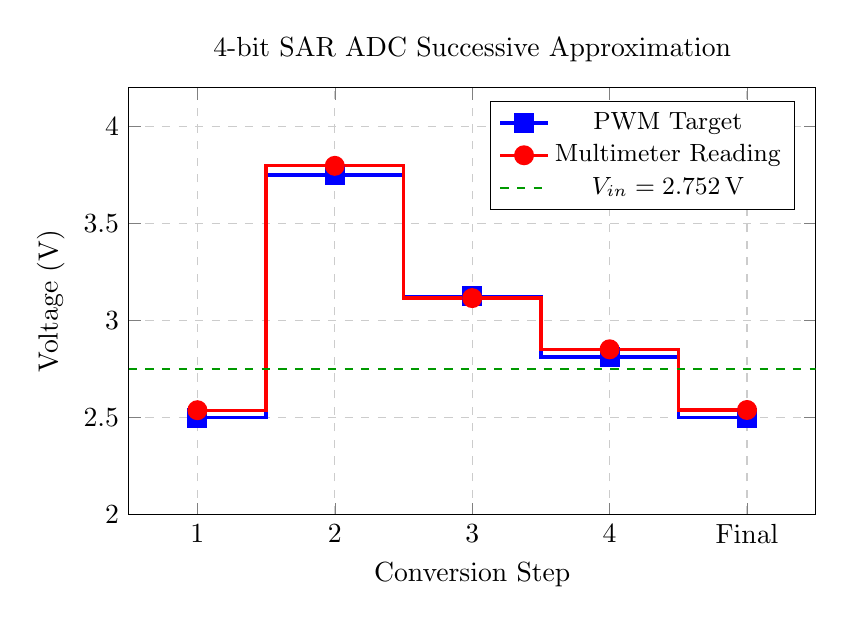
\begin{tikzpicture}
        \begin{axis}[
            width=0.85\textwidth,
            height=7cm,
            xlabel={Conversion Step},
            ylabel={Voltage (V)},
            title={4-bit SAR ADC Successive Approximation},
            xmin=0.5, xmax=5.5,
            ymin=2.0, ymax=4.2,
            xtick={1,2,3,4,5},
            xticklabels={1,2,3,4,Final},
            grid=major,
            grid style={dashed, gray!40},
            legend pos=north east,
            legend style={font=\small},
            const plot mark mid,
        ]
        % Staircase plot - PWM Target
        \addplot[blue, very thick, const plot mark mid, mark=square*, mark size=3pt]
            coordinates {(1,2.500) (2,3.750) (3,3.125) (4,2.812) (5,2.500)};
        \addlegendentry{PWM Target}
        
        % Staircase plot - Multimeter
        \addplot[red, very thick, const plot mark mid, mark=*, mark size=3pt]
            coordinates {(1,2.538) (2,3.798) (3,3.116) (4,2.852) (5,2.539)};
        \addlegendentry{Multimeter Reading}
        
        % Reference line
        \addplot[green!60!black, thick, dashed, domain=0.5:5.5] {2.752};
        \addlegendentry{$V_{in} = 2.752$\,V}
        
        \end{axis}
    \end{tikzpicture}
    \caption{4-bit SAR ADC Staircase Progression}
    \label{fig:4bit_staircase}
\end{figure}

\subsection{10-bit SAR ADC Staircase}
\begin{figure}[H]
    \centering
    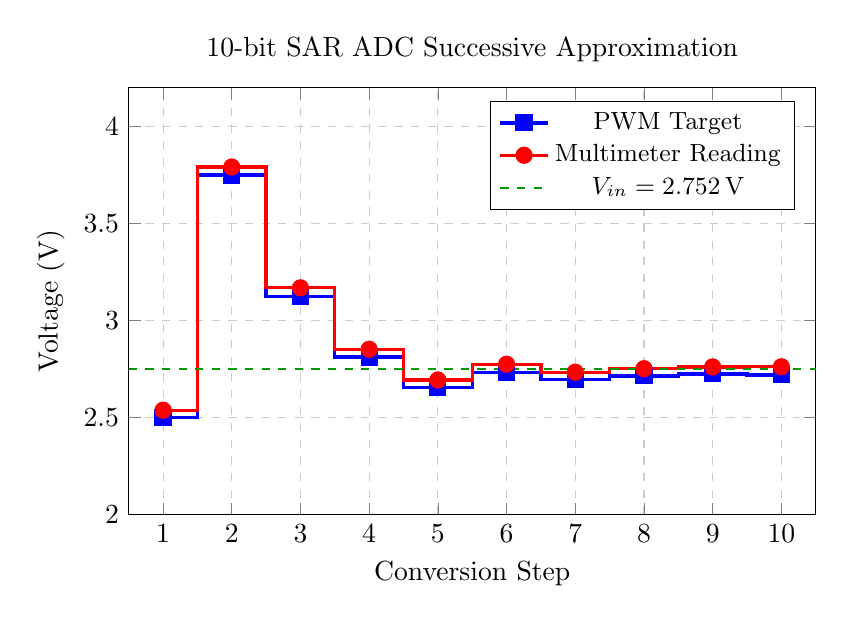
\begin{tikzpicture}
        \begin{axis}[
            width=0.85\textwidth,
            height=7cm,
            xlabel={Conversion Step},
            ylabel={Voltage (V)},
            title={10-bit SAR ADC Successive Approximation},
            xmin=0.5, xmax=10.5,
            ymin=2.0, ymax=4.2,
            xtick={1,2,3,4,5,6,7,8,9,10},
            grid=major,
            grid style={dashed, gray!40},
            legend pos=north east,
            legend style={font=\small},
        ]
        % Staircase plot - PWM Target
        \addplot[blue, very thick, const plot mark mid, mark=square*, mark size=2.5pt]
            coordinates {(1,2.500) (2,3.750) (3,3.125) (4,2.812) (5,2.656)
                         (6,2.734) (7,2.695) (8,2.715) (9,2.725) (10,2.720)};
        \addlegendentry{PWM Target}
        
        % Staircase plot - Multimeter
        \addplot[red, very thick, const plot mark mid, mark=*, mark size=2.5pt]
            coordinates {(1,2.538) (2,3.792) (3,3.169) (4,2.852) (5,2.694)
                         (6,2.775) (7,2.734) (8,2.752) (9,2.761) (10,2.762)};
        \addlegendentry{Multimeter Reading}
        
        % Reference line
        \addplot[green!60!black, thick, dashed, domain=0.5:10.5] {2.752};
        \addlegendentry{$V_{in} = 2.752$\,V}
        
        \end{axis}
    \end{tikzpicture}
    \caption{10-bit SAR ADC Staircase Progression}
    \label{fig:10bit_staircase}
\end{figure}

% --- ANALYSIS ---
\section{Experimental Analysis}

\subsection{Duty Cycle \& Mean Voltage Verification}
At the conclusion of the 10-bit conversion, the PWM signal was captured via oscilloscope to verify the relationship between the digital logic and the analog output. Figure~\ref{fig:duty_cycle} shows the oscilloscope capture.

\begin{figure}[H]
    \centering
    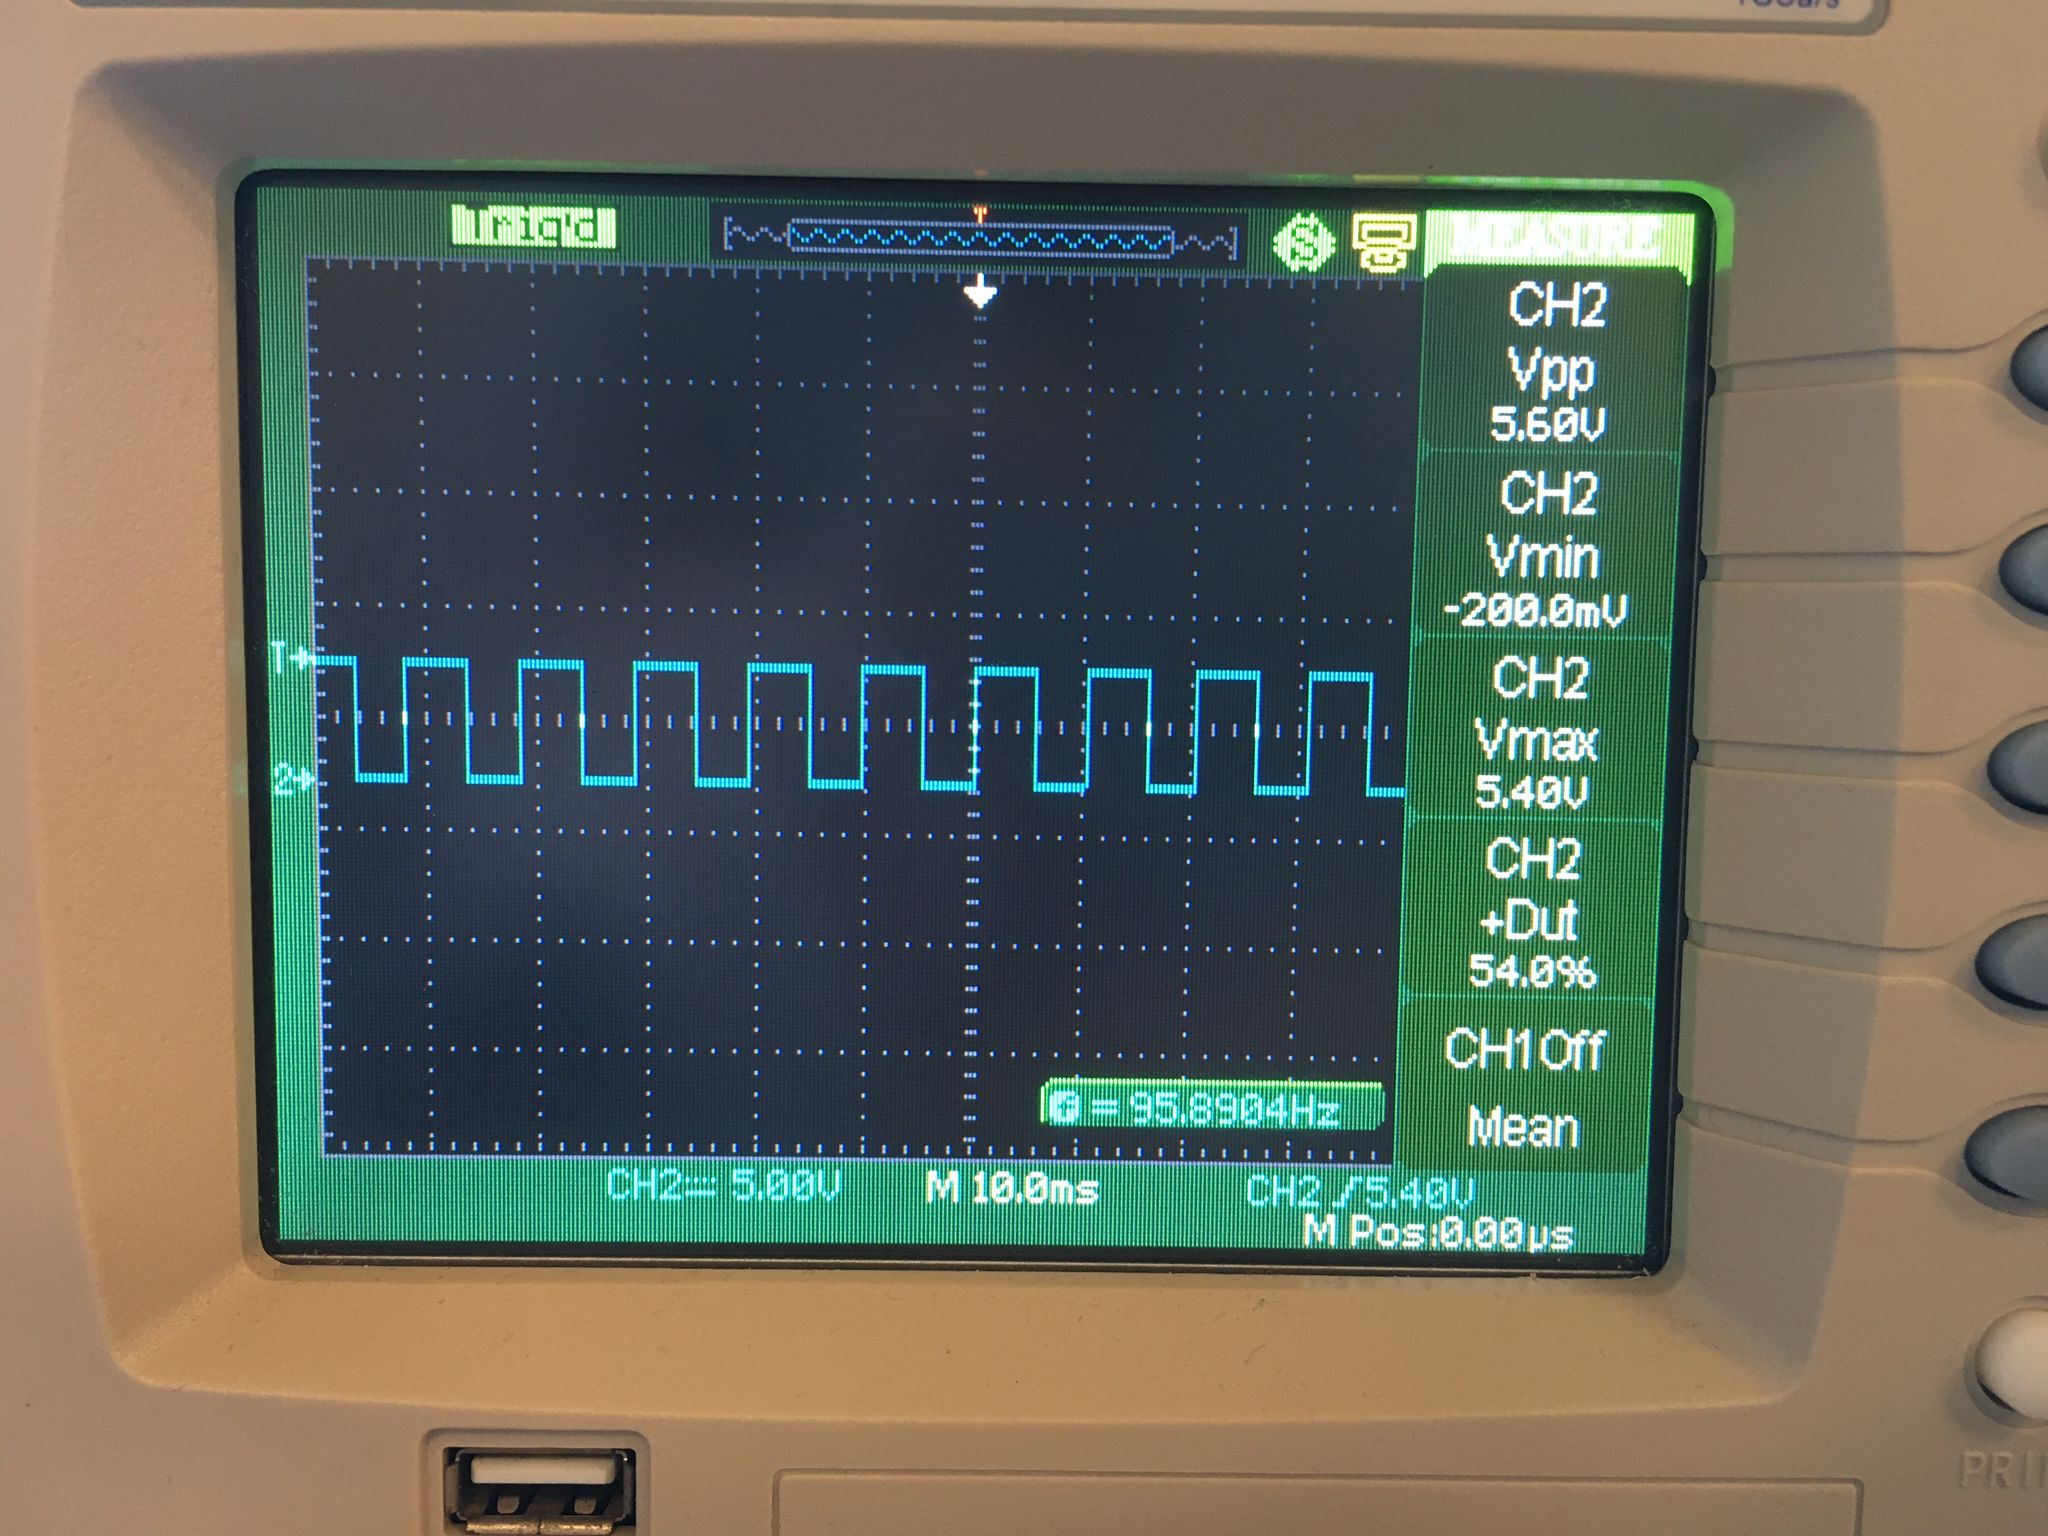
\includegraphics[width=0.75\textwidth]{images/duty_cycle.png}
    \caption{Oscilloscope capture of the final-step PWM signal showing a 54.0\% duty cycle.}
    \label{fig:duty_cycle}
\end{figure}

\begin{itemize}
    \item \textbf{Measured Duty Cycle ($D$):} 54\%
    \item \textbf{Supply Voltage ($V_{supply}$):} 5.00\,V
    \item \textbf{Calculated Mean Voltage:}
    \[
        V_{mean} = D \times V_{supply} = 0.54 \times 5.0\,\text{V} = 2.70\,\text{V}
    \]
\end{itemize}

The proximity of this calculated result to the 2.752\,V input confirms that the SAR controller effectively modulated the PWM to balance the inputs of the MCP6022 comparator. The slight difference between the calculated mean voltage (2.70\,V) and the actual capacitor voltage (2.762\,V) is attributed to the inherent ripple of the RC filter and the finite resolution of the oscilloscope's duty cycle measurement.

\subsection{Accuracy Evaluation}

\begin{table}[H]
    \centering
    \caption{Accuracy comparison of 4-bit and 10-bit SAR ADC results.}
    \label{tab:accuracy}
    \begin{tabular}{cccc}
        \toprule
        Mode & $V_{in}$ (V) & Final Estimate (V) & Absolute Error (V) \\
        \midrule
        4-bit  & 2.752 & 2.539 & 0.213 \\
        10-bit & 2.752 & 2.762 & 0.010 \\
        \bottomrule
    \end{tabular}
\end{table}

The 10-bit ADC reduces the absolute error from 213\,mV to just 10\,mV---a factor of $\sim$21$\times$ improvement. This clearly demonstrates that increasing the bit depth enables the SAR algorithm to converge much more closely to the true input voltage.

\subsection{Total Unadjusted Error (TUE)}
The TUE is calculated as the absolute difference between the true input voltage and the final ADC estimate. The theoretical quantization step size (1 LSB) and maximum quantization error for each resolution are:
\[
    \text{LSB}_{4} = \frac{5.0}{2^4} = 312.5~\text{mV}, \qquad Q_{e,max} = \frac{\text{LSB}}{2} = 156.25~\text{mV}
\]
\[
    \text{LSB}_{10} = \frac{5.0}{2^{10}} = 4.883~\text{mV}, \qquad Q_{e,max} = \frac{\text{LSB}}{2} = 2.441~\text{mV}
\]

\begin{table}[H]
    \centering
    \caption{Total Unadjusted Error comparison.}
    \label{tab:tue}
    \begin{tabular}{cccc}
        \toprule
        Mode & TUE (mV) & Theoretical $Q_{e,max}$ (mV) & TUE / LSB \\
        \midrule
        4-bit  & 213.0 & 156.25 & 0.68 \\
        10-bit & 10.0  & 2.441  & 2.05 \\
        \bottomrule
    \end{tabular}
\end{table}

For the 4-bit ADC, the TUE of 213\,mV falls within 1 LSB (312.5\,mV), which is consistent with the theoretical quantization limit. The error is primarily dominated by the coarse resolution of the 4-bit system. For the 10-bit ADC, the TUE of 10\,mV exceeds the theoretical quantization floor (2.441\,mV) by approximately 2 LSBs, indicating that analog error sources---primarily the RC filter settling time ($\tau = 47~\text{k}\Omega \times 10~\mu\text{F} = 0.47$\,s) and the comparator's input offset voltage---contribute to the residual error at this resolution.

% --- CONCLUSION ---
\section{Conclusion}
The laboratory experiment successfully demonstrated the implementation of a SAR ADC using an Arduino-based PWM-to-DC conversion technique. The convergence data and duty cycle measurements confirm that the binary search algorithm functions correctly, narrowing the error margin with each successive bit.

The 4-bit conversion yielded a final estimate of 2.539\,V with an absolute error of 213\,mV, while the 10-bit conversion reached 2.762\,V with an error of only 10\,mV. The staircase progression plots clearly illustrated the non-monotonic, zig-zag nature of the SAR algorithm, and the 10-bit zoomed view showed how the estimate oscillates around the true input with diminishing amplitude.

Although the 10-bit resolution provides a theoretical quantization floor of 4.88\,mV, practical analog imperfections such as RC filter settling and comparator sensitivity set the final precision limit at 10\,mV in this implementation. This demonstrates that while increasing bit depth significantly improves accuracy, the analog front-end must also be optimized to fully exploit the available digital resolution.

\end{document}